In this chapter we will show how we have implemented the architectures presented in chapter \ref{chapter:architectures}.

\section{Testing Programs}
We have developed an application for testing computation offloading. It is easily configurable and flexible for testing. The next two subsections will show how it is implemented.

\subsection{Computation offloading}
For computation offloading we initially wanted to implement Eratosthenes Sieve for finding primes. This is because it has an interesting way parallelizing, and therefore distributing the work. However, due to an limitation from the Emerald VM, memory runs out when trying to find primes higher than a million. Memory use of the algorithm can be optimized, but it does not change the fact that Eratosthenes Sieve is a memory intensive algorithm. Therefore we are doing hashing instead. Hashing is a low memory, compute intensive task. This is excellent for our simulation as we primarily want to focus on computational use and latency.






\subsection{Classes and structure}
\begin{figure}[t]
    \centering
    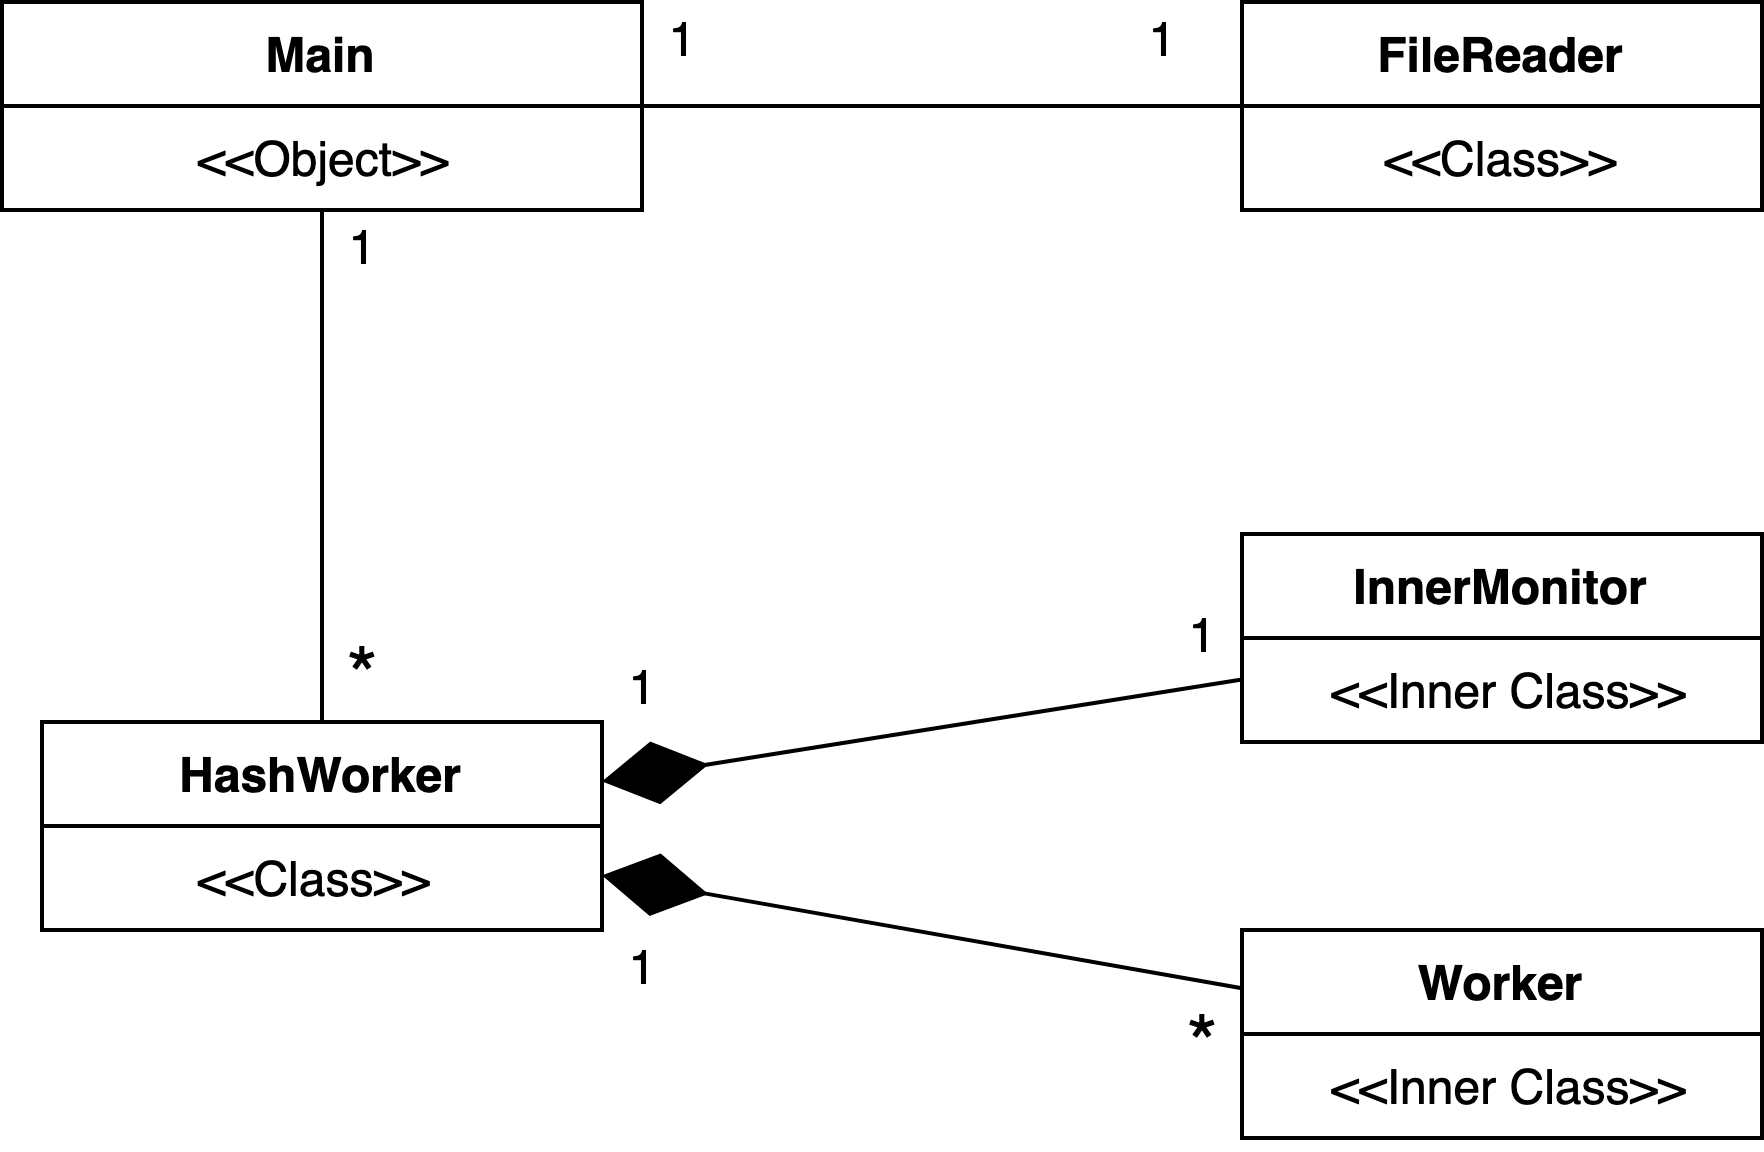
\includegraphics[scale=0.9]{chapters/implementation/figures/HashWorker_class_diagram.png}
    \caption{Illustration of the class structure used for computation offloading}
    \label{fig:HashWorker_class_diagram}
\end{figure}
Figure \ref{fig:HashWorker_class_diagram} shows the class structure. We have four classes and one object. We will now go through each of them and briefly explain what they do.


%Mention that since InternalMonitor has fields, getters and setters are automatically created at compile time, and since it is in a monitor, it is guaranteed that only one thread at a time can call those functions. 


\subsubsection{FileReader}
Below is the interface of class FileReader:
\begin{lstlisting}[language=emerald]
const FileReader <- class FileReader
  export op readFile[fileName: String] 
                            -> [res: Array.of[String]]
                            
  export function convertConfigToIntegers
                            [input: Array.of[String]] 
                          -> [res: Array.of[Integer]]
                            
  function stripLast[i: String] -> [o: String]
end FileReader
\end{lstlisting}
The operation \verb|readFile| will read the file with the path provided in parameter \verb|fileName|. For each line it reads, it will delete the last character with \verb|stripLast|, as it is a unwanted newline character. The function \verb|convertConfigToIntegers| is a function that converts an array of strings to an array of integers. This is needed because configs consists of lines of numbers, but they are read as strings.



\subsubsection{HashWorker}
Below is the interface of class HashWorker:
\begin{lstlisting}[language=emerald]
const HashWorker <- class HashWorker
                                [limitation: Integer]
  
  attached const workload %String

  attached const mon <- InnerMonitor.create

  attached const InnerMonitor 
                        <- monitor class InnerMonitor

  attached const Worker
                  <- class Worker[iterations: Integer]

  initially

  export op setLimitation[lim: Integer]
  
  export op doWork[iterations: Integer, 
                    work: LocalWorkload, 
                    frequencyOfGet: integer]

  export op collectTimeUsed -> [res: Time]
end HashWorker
\end{lstlisting}
HashWorker is an object that is distributed to all machines. The role of HashWorker is to provide an interface for main to start and control work. The constant \verb|mon| is used to store an instance of the \verb|InnerMonitor| class. Then we have the definitions for \verb|InnerMontor| and \verb|Worker|. They are defined inside the HashWorker class and are therefore inner classes. Then we have the \verb|initially| section. Here we ensure that the class parameter \verb|limitation| is equal to or higher than zero. This is because the limitation is used to make a time constraint, and we don´t want negative time. Operation \verb|setLimitation| is there to be able to change the limitation during runtime. Operation \verb|doWork| will create an instance of the \verb|Worker| class. It takes a parameter \verb|iterations| which is how many iterations we want the node to do, \verb|work| which is the workload that the worker will hash, and \verb|frequencyOfGet| which is how often we retrieve information from Local (the mobile device). Operation \verb|collectTimeUsed| is used to collect the time used after process is done. When called, it will wait for the process in Worker to be done, then return the time used.
Notice that all of the constants are attached. This is because we want to ensure that all of them are on the same node as the HashWorker instance. This reduces the amount of costly remote reads.




\subsubsection{InternalMonitor}
Below is the whole class of InnerMontor:
\begin{lstlisting}[language=emerald]
attached const InnerMonitor 
                        <- monitor class InnerMonitor
  field waiting : Boolean <- true

  field timeTaken : Time <- nil
end InnerMonitor
\end{lstlisting}
As discussed in section \ref{emerald:field}, fields in Emerald automatically generates getters and setters. Since it is in a monitor class it is guaranteed that invoking them is mutual exclusive. In other words, the getters and setters that are automatically created within the class is safe to use in parallel. Variable \verb|timeTaken| is used to store the time used by the process in class \verb|Worker|. Variable \verb|waiting| is used to ensure that main does not collect \verb|timeTaken| before the worker is done. 





\subsubsection{Worker}
Below is the skeleton of class Worker.

\begin{minipage}{\linewidth}
\begin{lstlisting}[language=emerald]
attached const Worker 
                <- class Worker[iterations: Integer]
                
    initially
    
    process
    
    function djb2Hash[str: String] -> [res: Integer]
end Worker
\end{lstlisting}
\end{minipage}
The \verb|initially| section will assert that iterations are higher than zero, because we should avoid doing negative amount of work. The \verb|process| section is where the actual work of the node happens. When \verb|doWork| is called in class \verb|HashWorker|, it creates an instance of the Worker class by invoking operation \verb|create|. The process is then started. In the process, it will run parameter \verb|iterations| number of iterations. The hashing algorithm we use is called \textit{Djb2}. Our implementation is a converted version from a C implementation found here\cite{noauthor_hash_nodate}. 
\begin{lstlisting}[language=emerald]
function djb2Hash[str: String] -> [res: Integer]
  res <- 5381
  for i : Integer <- 0 while i < str.length 
                                    by i <- i + 1
    res <- res * 33 * str[i].ord
  end for
end djb2Hash
\end{lstlisting}
The algorithm takes a string, iterates over it and multiplies itself with 33 and the characters ordinal number. To make it even more compute heacy, we convert the result to string, and then re-insert that into the hash function 10000 times. We see that as one iteration, as shown in figure \ref{fig:Hashing_algorithm_iteration}. In other words, the HashWorker will do what figure \ref{fig:Hashing_algorithm_iteration} shows, parameter \verb|iterations| number of times. Since we just throw out the result after each time, Emeralds garbage compiler will ensure that we have plenty of memory available. 
\begin{figure}[t]
    \centering
    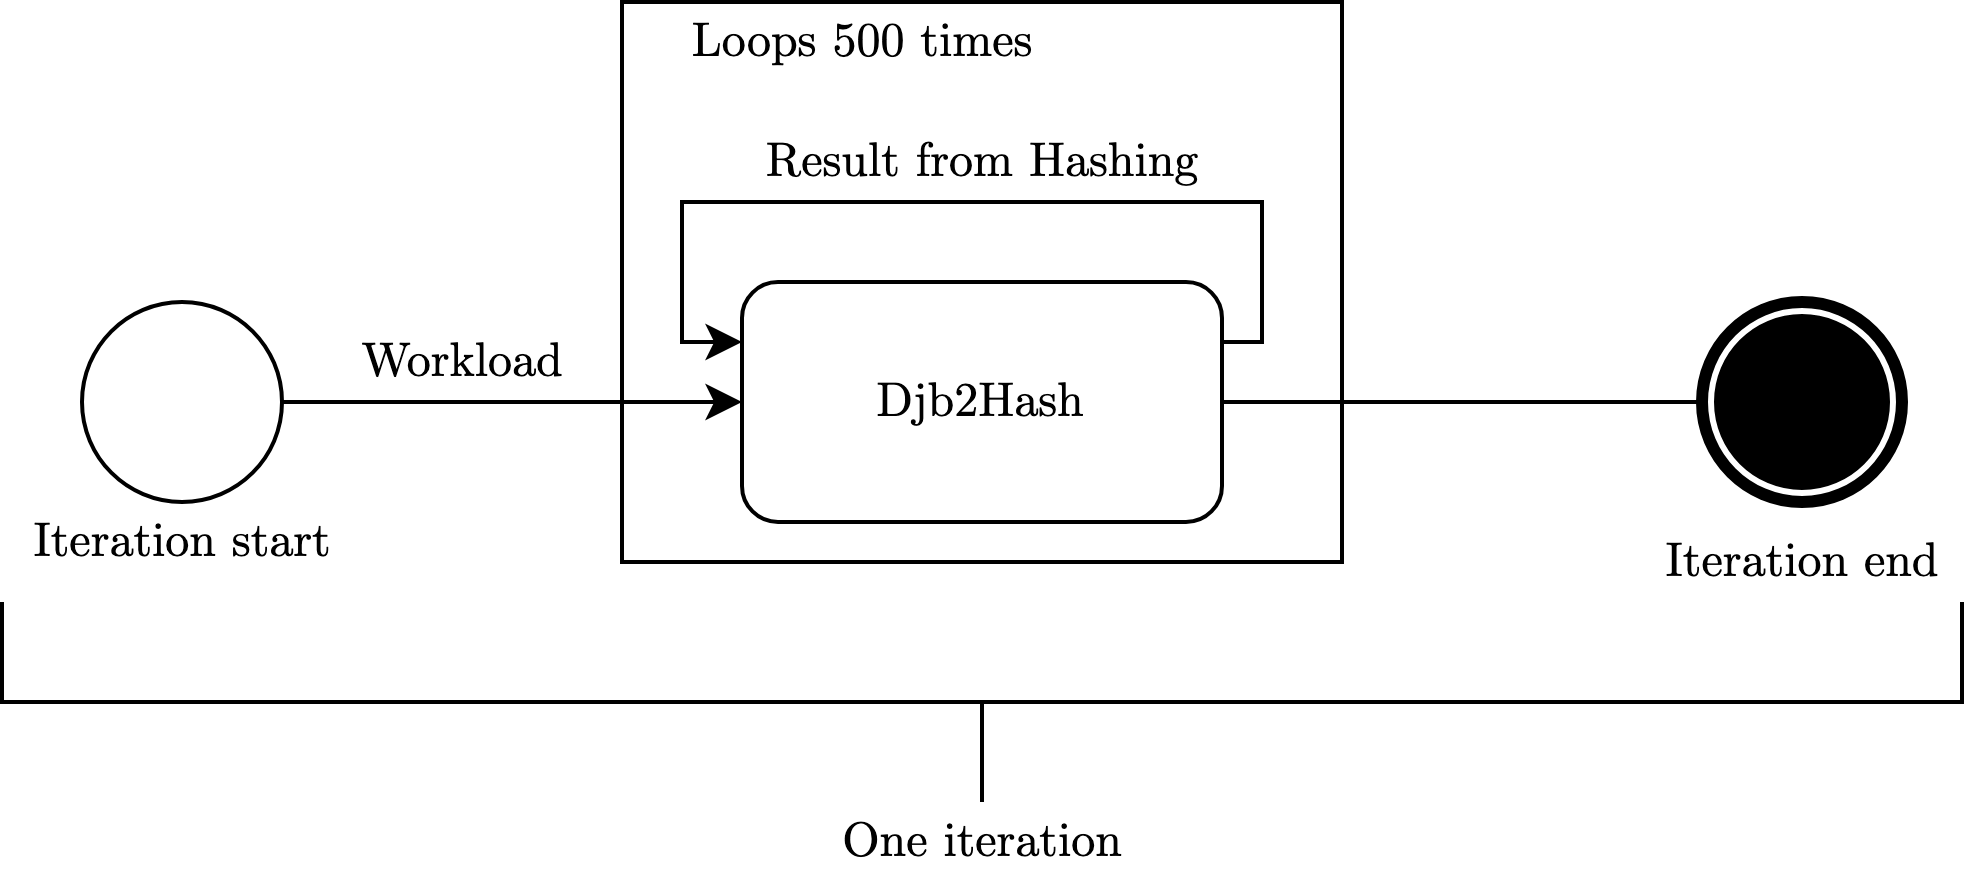
\includegraphics[scale=0.9]{chapters/implementation/figures/Iteration.png}
    \caption{Illustration of one iteration in the HashWorker}
    \label{fig:Hashing_algorithm_iteration}
\end{figure}
In each iteration it will also check if we have to get information from Local, as well as taking the time on how long we do calculations and how long we wait for response.



\subsubsection{Main}
Main only has an initially section that will do a number of steps. First it will move through all nodes and print some information on each node. This is mainly for debugging, and to ensure that things are running correctly. Further it will invoke the create an instance of the \verb|FileReader| class and read config file that you have specified. Config files are discussed in subsection \ref{subsection:configfiles}. Further, it will use this config to initilize \verb|HashWorker| instances and move them to a node decided by user input. Then, it will iterate through all \verb|HashWorker| instances and invoke operation \verb|doWork|. All processes should then have started. Finally, it will collect and print the results.



\subsection{Simulating CPU restrictions}
To simulate CPU restrictions, we place a limitation on each HashWorker. To be able to accurately control how much work is done on each HashWorker, we have implemented a way of specifying how many iterations (see figure \ref{fig:Hashing_algorithm_iteration}) each node can do per second.



\subsection{Config files}\label{subsection:configfiles}
When the \verb|FileReader| class reads in the config file, it expects a very simple syntax. Each line should be a positive integer. For example a file that for two HashWorkers will set their limitations to 0 and 100 and make them both do 50 iterations, and make them get from Local with a frequency of 1 and 30 iterations, will look like this:
\begin{lstlisting}
0
100
1
30
50
50

\end{lstlisting}
The \verb|FileReader| reads each line until the newline character. The config file is terminated by an emtpy line at the end. After everything is read, it will convert them to an array of Integers, instead of array of Strings.

\subsection{Placing HashWorkers}
Placement of HashWorkers is prompted in the terminal. When testing you will get information about an HashWorker, and a choice for which node you want to place it on. 














% -----------------------------------------------------------------------------------

\section{Multi-Access Edge Computing}

\begin{figure}[t]
    \centering
    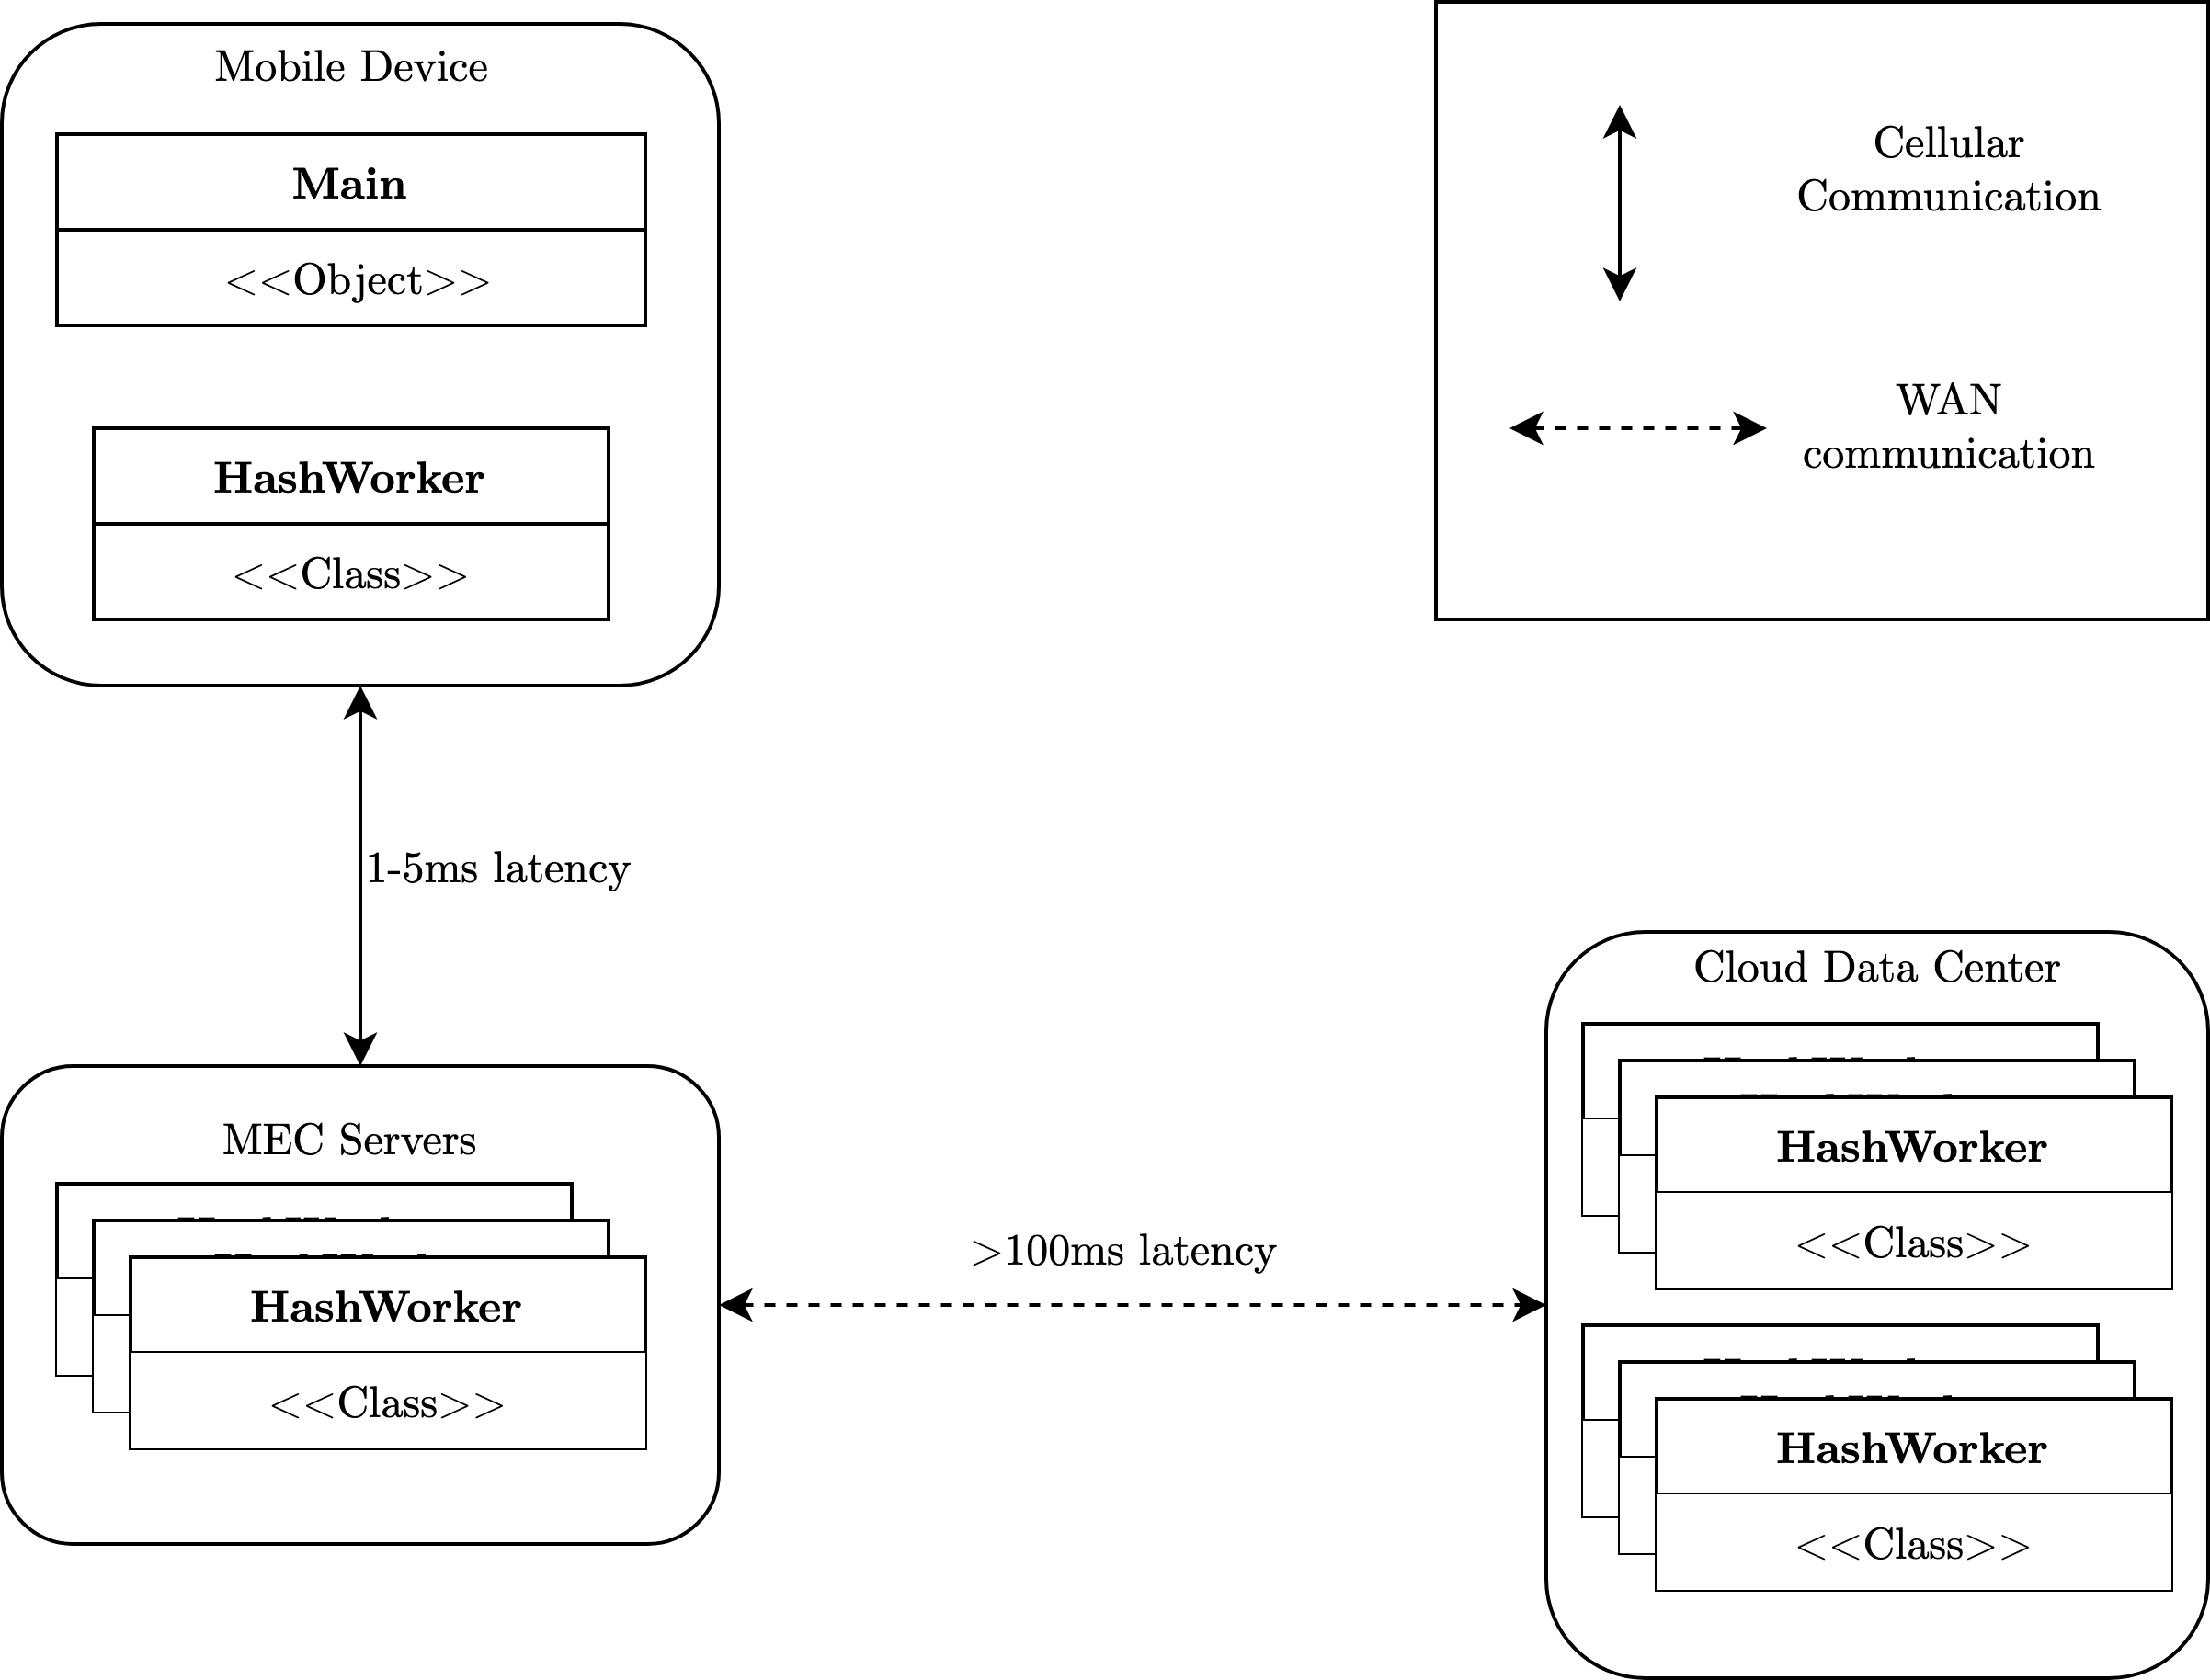
\includegraphics[scale=1]{chapters/implementation/figures/MEC_implementation.png}
    \caption{Illustration of the node structure used for computation offloading in MEC}
    \label{fig:MEC_implementation}
\end{figure}
Figure \ref{fig:MEC_implementation} illustrates how three nodes can be set up. The \verb|Main| object will reside on the mobile device, as that is where we want the result. We can create several HashWorkers to place them on servers. However, the Cloud Data Center will have enough resources to have significantly more HashWorkers than the MEC Servers, and the MEC Servers can have significantly more HashWorkers than the mobile client. The MEC Servers can consist of one or more machines that hosts one to many HashWorker instances. The Cloud Data Center consists of many machines that can host one to many HashWorker instances.




% -------------------------------------------------------------------

\section{Cloudlets}
\begin{figure}[t]
    \centering
    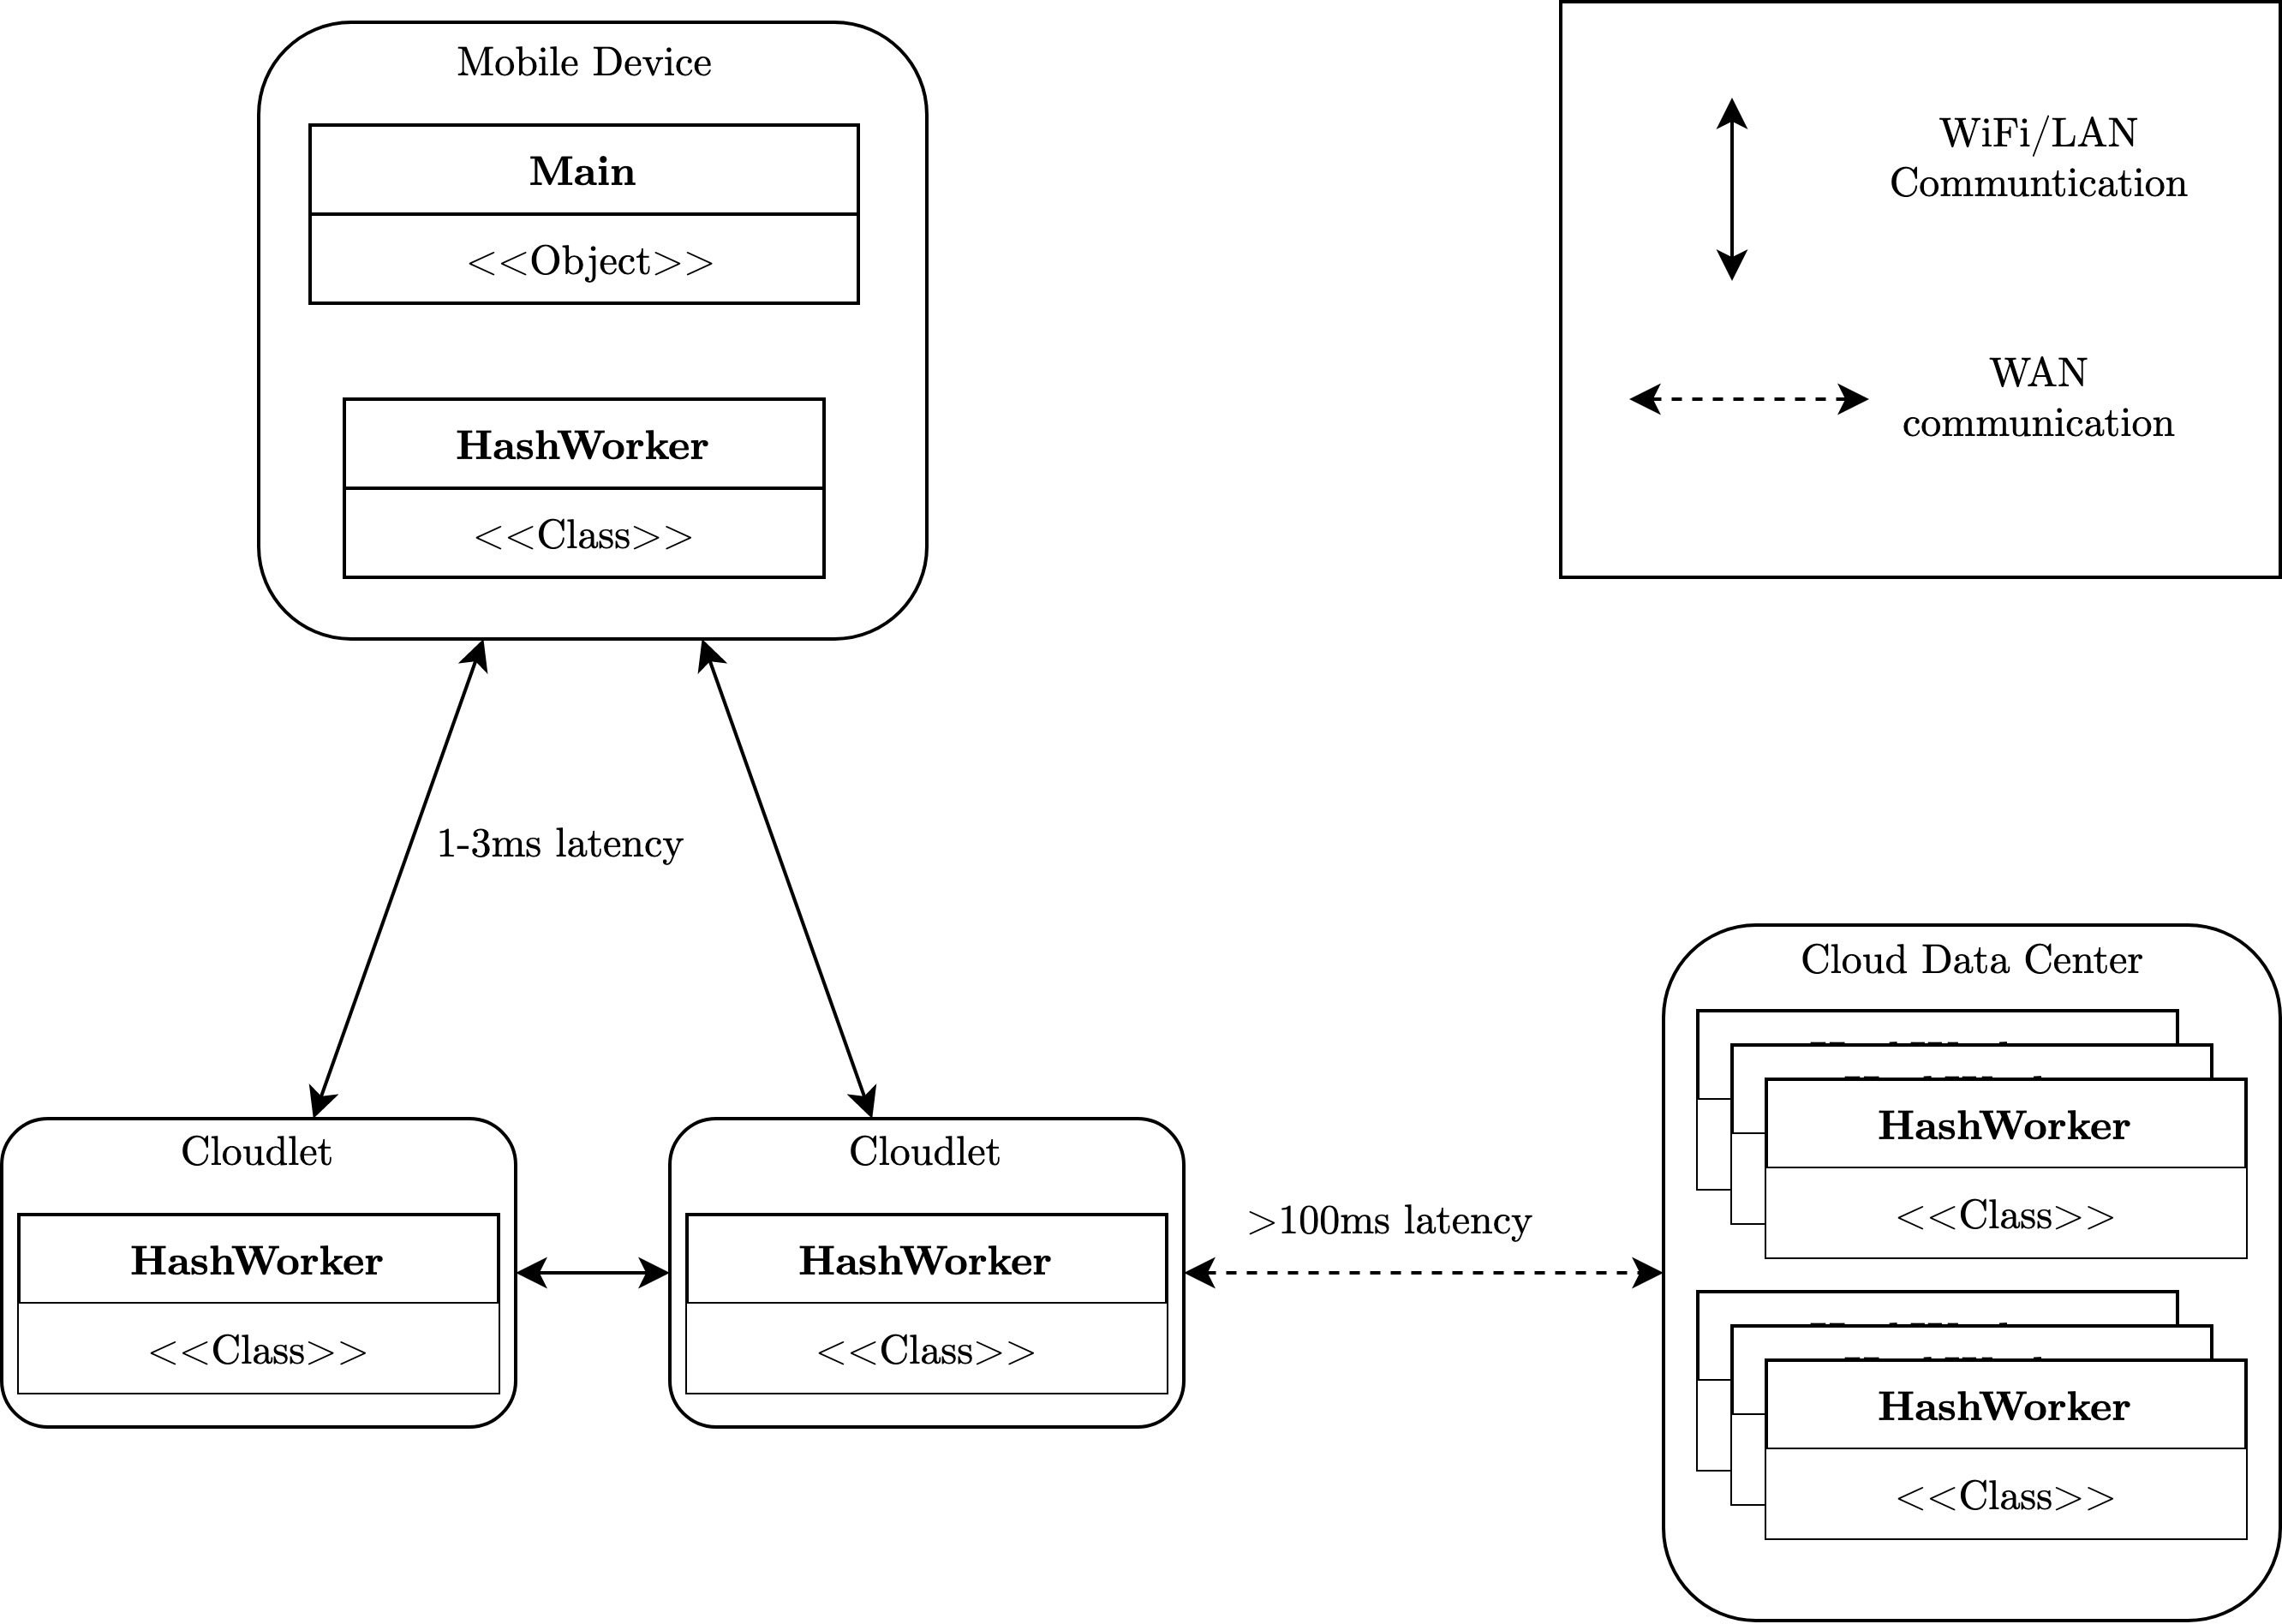
\includegraphics[scale=0.9]{chapters/implementation/figures/Cloudlet_implementation.png}
    \caption{Illustration of the node structure used for computation offloading with Cloudlets}
    \label{fig:Cloudlet_implementation}
\end{figure}
Figure \ref{fig:Cloudlet_implementation} illustrates how we can set up an example implementation of Cloudlets. The mobile device will be in very short distance of the Cloudlets and therefore use WiFi to connect with them. In our tests, the Cloudlets are not access points themselves, and therefore there is a WiFi accesspoint hop between the mobile device and the Cloudlets.










\section{Summary}
In this chapter we have described the prototype we have created. The prototype can easily be setup with configuration files to control different parameters for each worker on each node. This lets us easily set up high-level simulations of Near-Far architectures and models. Additionally we have provided some examples of how you can use it to model Cloudlets and Mobile Edge Computing.